\documentclass[margin,line]{resume}
\usepackage[hidelinks]{hyperref}
\usepackage{tikz}
\setlength{\textheight}{9.7in}
\newenvironment{absolutelynopagebreak}
  {\par\nobreak\vfil\penalty0\vfilneg
   \vtop\bgroup}
  {\par\xdef\tpd{\the\prevdepth}\egroup
   \prevdepth=\tpd}

\begin{document}
\begin{tikzpicture}
\clip (0,0) circle (1cm) ;
\node[anchor=center] at (0,0) {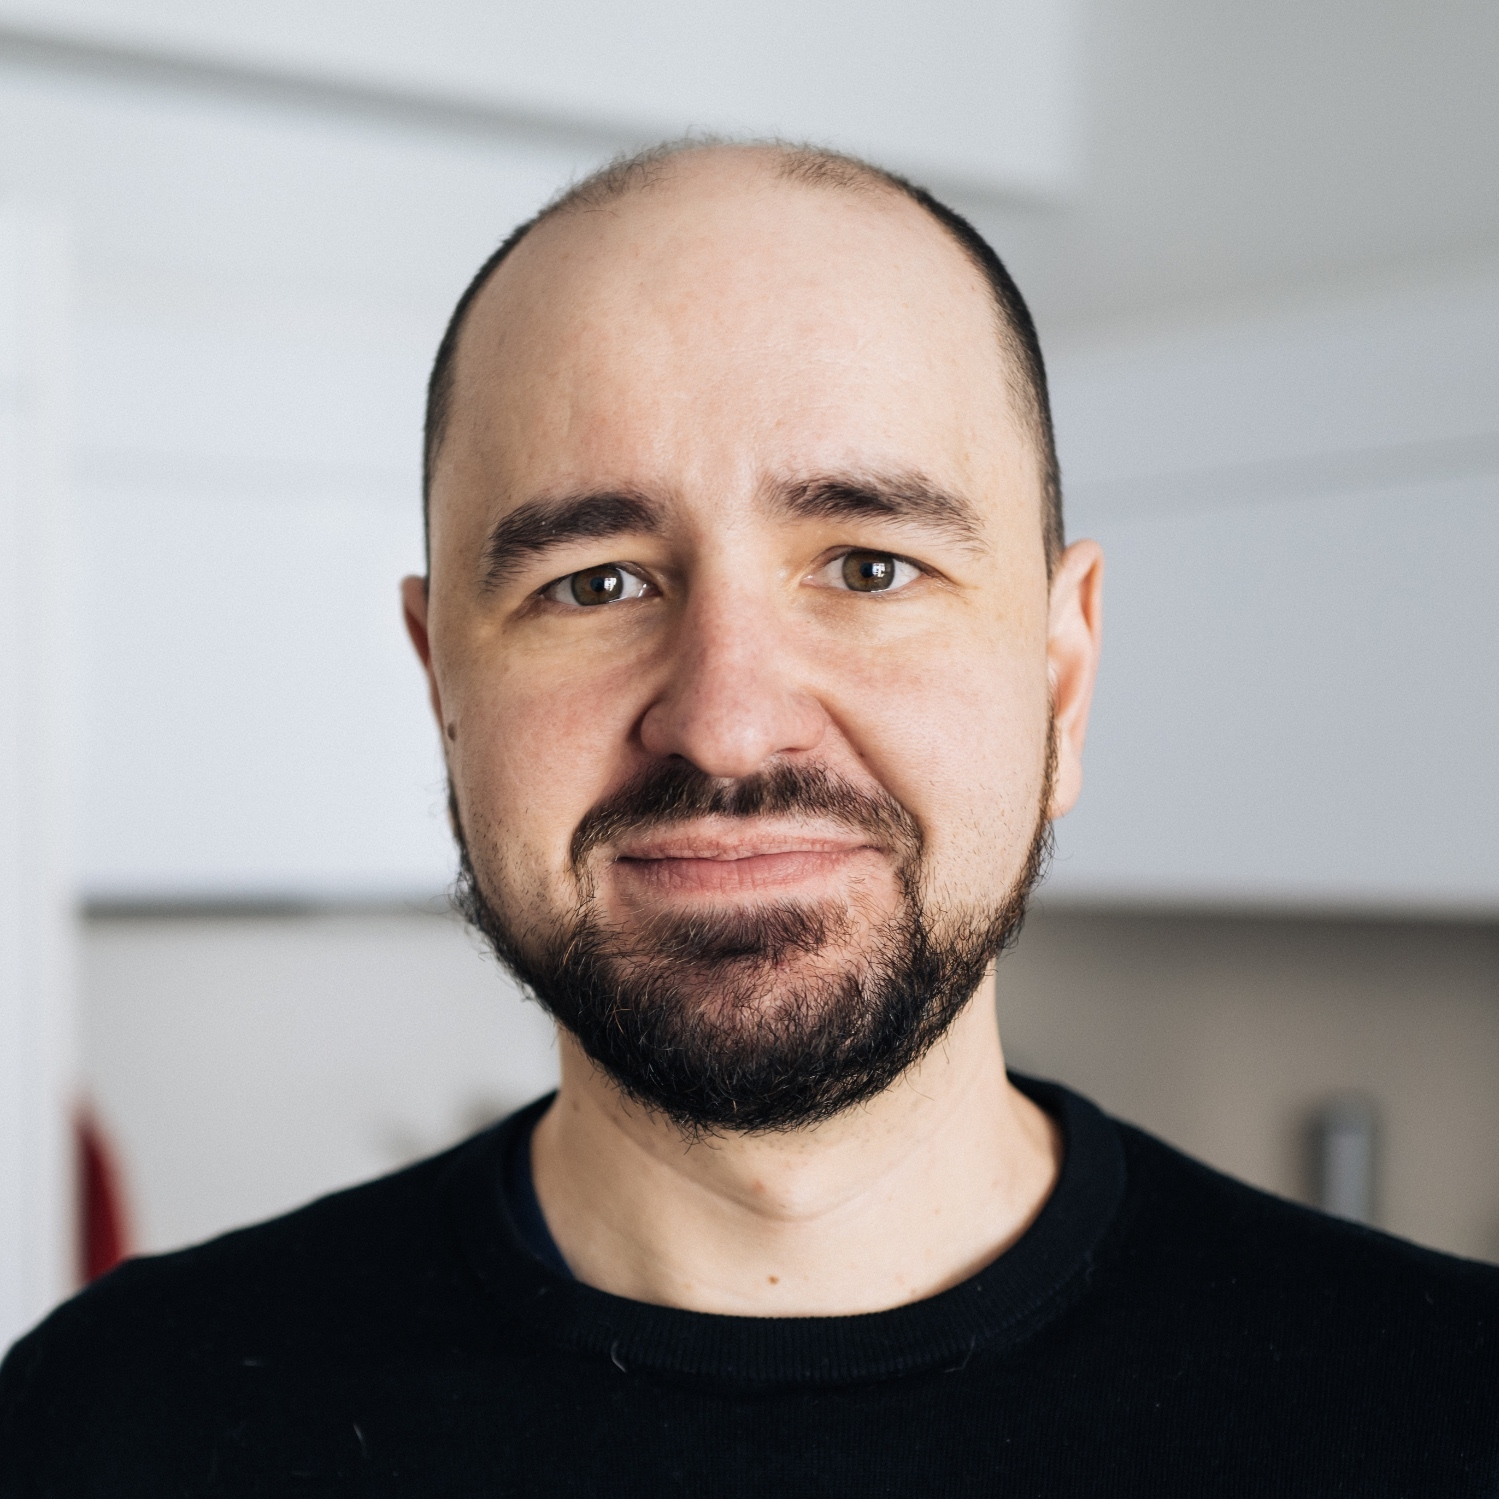
\includegraphics[width=2cm]{myface}};
\end{tikzpicture} \name{\Large Brenden Matthews}
\begin{resume}

    \section{\mysidestyle Contact\\Information}

    Email: \href{mailto:resume@brenden.brndn.io}{\texttt{resume@brenden.brndn.io}} \hfill
    GitHub: \href{https://github.com/brndnmtthws}{\texttt{github.com/brndnmtthws}} \hfill
    Website: \href{https://brndn.io}{\texttt{brndn.io}} \hfill
    \vspace{3mm}

    \section{\mysidestyle Published\\Works}

    \href{https://www.manning.com/books/code-like-a-pro-in-rust}{\textbf{Code Like a Pro in Rust}}, Manning Publications. ISBN 9781617299643.
    \linebreak \href{https://www.manning.com/books/rust-design-patterns}{\textbf{Rust Design Patterns}}, Manning Publications,
    estimated summer 2024. ISBN 9781633437463.

    \vspace{3mm}

    \section{\mysidestyle Public\\Speaking}

    Have given numerous talks on my work at conferences and private engagements,
    including but not limited to \textbf{All Things Open}, \textbf{QCon},
    \textbf{LinuxCon}, \textbf{ContainerCon}, and \textbf{MesosCon}.

    \vspace{3mm}

    \section{\mysidestyle Open\\Source}

    Contributed to hundreds of open source projects including Apache Airflow,
    Apache Kafka, Apache Superset, Apache Spark, Apache Mesos (PMC member), . Member of the
    Apache Software Foundation. Personally created a number of popular projects,
    with a few highlighted below:

    \href{https://github.com/brndnmtthws/conky}{\textbf{Conky}}, C and C++ \hfill \textbf{6.9k+ stars}\\
    Endlessly configurable system monitor utility for UNIX systems.

    \href{https://github.com/brndnmtthws/thetagang}{\textbf{ThetaGang}}, Python \hfill \textbf{1.8k+ stars}\\
    Equity options trading tool for capturing premium from theta decay. Designed
    for use with IBKR.

    \href{https://github.com/brndnmtthws/dryoc}{\textbf{dryoc}}, Rust \hfill \textbf{230+ stars}\\
    High quality pure-Rust general purpose cryptography library compatible with
    libsodium.  Features generic hash functions suitable for cryptography,
    protected memory, zeroization, and SIMD.

    \vspace{3mm}

    \begin{absolutelynopagebreak}
    \section{\mysidestyle Professional\\Experience}

    \textbf{Entrepreneur, Author, Consultant}, New York, NY\hfill \textbf{May 2019 -- present}\vspace{2mm}\\\vspace{1mm}%
    \begin{itemize}
        \item Started several bootstrapped businesses
        \item Engaged in a mix of consulting work
        \item Wrote two books on Rust programming
        \item Contributed to a number of open source projects
        \item Gave a number of talks at meetups
    \end{itemize}
    \end{absolutelynopagebreak}

    \vspace{5mm}

    \begin{absolutelynopagebreak}
    \textbf{Braze, Inc.}, New York, NY\hfill \textbf{Oct 2018 -- April 2019}\vspace{2mm}\\\vspace{1mm}%
    \textsl{Engineering}

    Building infrastructure with Kubernetes.
    
    \begin{itemize}
        \item Lead an effort to transform ad-hoc Bash-based deployment scripts
        into declarative Helm and Terraform based deployments
        \item Provided engineering-wide guidance and training for migrating to
        Terraform and Helm
        \item Ported primary Rails monolith to Kubernetes
        \item Implemented continuous integration and deployment system for
        Kubernetes applications
    \end{itemize}
    \end{absolutelynopagebreak}

    \vspace{5mm}

    \begin{absolutelynopagebreak}
    \textbf{Citadel LLC}, New York, NY\hfill \textbf{Oct 2017 -- Jun 2018}\vspace{2mm}\\\vspace{1mm}%
    \textsl{Engineering}

    Joined the platform engineering group as part of the data engineering
    team to build out Citadel's data platform technology. Primarily working
    with tools that integrate on-prem and cloud (AWS and GCE) data
    infrastructure.

    \begin{itemize}
        \item Lead an effort to modernize data access, control, and
        authorization
        \item Managed a migration of legacy data systems to PostgreSQL on RDS
        backends
        \item Provided technical leadership to the data science team for best
        practices on building and deploying very large machine learning jobs
        with Spark, Redshift, and Snowflake
    \end{itemize}
    \end{absolutelynopagebreak}

    \vspace{5mm}

    \begin{absolutelynopagebreak}
    \textbf{D2IQ (fka Mesosphere), Inc.}, San Francisco, CA\hfill \textbf{Jan 2015 -- Feb 2017}\vspace{2mm}\\\vspace{1mm}%
    \textsl{Sales \& Engineering}

    As an early Mesosphere employee, was an integral part of founding the
    company.  Worked on multiple customer engagements, acting in both pre-sales
    and post-sales positions. Assisted management with fundraising pitches.

    \begin{itemize}
        \item Built the initial sales team by leading key hires for VP Sales,
        early SEs, SAs, and Head of Services
        \item Built cloud migration plans for enterprise customers
        \item Lead and lectured week-long in-depth onsite training sessions
        \item Advised C-level management at Fortune 500 companies on container
        technology adoption to accelerate their innovation
        \item Lectured and gave talks at several meetups and conferences
        \item Contributed to various engineering efforts
        \item Published several original blog posts
        \item Built and maintained marathon-lb, the canonical load balancing and
        service discovery tool for Marathon and DC/OS
    \end{itemize}
    \end{absolutelynopagebreak}

    \vspace{5mm}

    \begin{absolutelynopagebreak}
    \textbf{Airbnb, Inc.}, San Francisco, CA\hfill \textbf{Feb 2013 -- Jan 2015}\vspace{2mm}\\\vspace{1mm}%
    \textsl{Engineering}

    Early employee at Airbnb. Joined the Data Infrastructure team to help
    Airbnb scale to support the massive growth of the company, and meet the
    company's needs for managing a large, growing data warehouse. Worked
    directly with teams all across the company to help meet their data needs,
    and build out a rich set of data tooling.

    \begin{itemize}
        \item Built next generation of data infrastructure utilizing open source
        tools such as Mesos, Hadoop, HDFS, Chronos, and Storm
        \item Contributed code to several projects, including: Mesos, Hadoop,
        Storm, Spark, Presto, Chronos, Marathon, and others
        \item Worked on early versions of Apache Superset (fka Airpal)
        \item Lead work on next generation of data processing tools, including
        Apache Airflow
        \item Lead an effort to improve data quality through the use of an
        automated verification system
        \item Coined our team motto of \emph{"Provably correct data"}
        \item Gave a number of internal tech talks on emerging technologies at
        Airbnb
    \end{itemize}
    \end{absolutelynopagebreak}

    \vspace{5mm}

    \begin{absolutelynopagebreak}
    \textbf{Newfield Wireless, Inc.}, Berkeley, CA\hfill \textbf{Sept 2009 -- Nov 2012}\vspace{2mm}\\\vspace{1mm}%
    \textsl{Engineering}

    Leveraged 3GPP layer 3 expertise to build a UMTS network data parser and
    indexer. Designed and implemented the first suite of real-time 3GPP LTE
    capture/parsing tools.

    \begin{itemize}
        \item Created a customized database solution with integrated flexible
        query language for accessing millions of streaming records in real-time
        \item Designed and implemented asynchronous communication library with
        feature set similar to ZeroMQ, with C++ and Python interfaces
        \item Designed and implemented a reporting library for generating key
        performance indicators from vast quantities of raw data, leveraging
        previously mentioned customized database
        \item Introduced new development and debugging methodologies to the team
        which significantly improved the pace of development and quality of
        deliverables
        \item Assisted junior and senior developers on all aspects of software
        engineering
        \item Oversaw design and implementation of schema-based XML software
        specifications
    \end{itemize}
    \end{absolutelynopagebreak}
    
    \vspace{5mm}

    \begin{absolutelynopagebreak}
    \textbf{Real Time Measurements, Inc.}, Calgary, AB\hfill \textbf{2003 -- 2009}\vspace{2mm}\\\vspace{1mm}%
    \textsl{Engineering}

    \begin{itemize}
        \item Developed end user applications, web services, and embedded
        software
        \item Involved in strategic planning, performance and productivity
        improvement, organizational design, e-commerce, new media and Internet
        promotion
        \item Planned, participated, and coordinated team building exercises
        while demonstrating strong leadership skills
        \item Configured and managed servers, automated backup systems, and
        provided support for customers as well as in-house support
        \item Leveraged new technologies to enhance our product-to-customer
        experience in a timely and cost effective fashion
        \item Implemented cost reduction IT strategy to make use of existing
        infrastructure instead of requiring further equipment purchases
    \end{itemize}
    \end{absolutelynopagebreak}

    \vspace{3mm}
    
    \section{\mysidestyle Programming\\Experience}

    \emph{Languages:} Rust, C, C++, Python, Ruby, Bash, Go, Java, Scala, Kotlin, \LaTeX \\
    \emph{Data Technology:} Kafka, Cassandra, Redis, PostgreSQL, ElasticSearch/Lucene,
     MySQL, Hadoop, Hive, Presto, RedShift, BigQuery, SQS, EMR, RDS, Snowflake,
     PyTorch, TensorFlow

    \section{\mysidestyle Authentication}

    The original source for this resume is available at
    \href{https://github.com/brndnmtthws/resume}{\texttt{github.com/brndnmtthws/resume}}.
    Use the contact email address at the top of this document or the one listed
    on my GitHub profile if you suspect shenanigans (such as fake candidates
    posing with my profile/details).
\end{resume}
\end{document}
